\subsection{Scenario 3}

\subsubsection{Configuration}

Pour voir ce qui se passe au niveau du contrôleur, on pourra si on le souhaite lancer une session wireshark sur l'interface concernée afin d'examiner les divers paquets Openflow transitant entre ONOS et switchs (notamment les paquets encapsulés en PACKET\_IN). Le filtre "tcp.port == 6633 \&\& openflow\_v4 \&\& (openflow\_v4.type == OFPT\_PACKET\_IN or openflow\_v4.type == OFPT\_PACKET\_OUT)" peut être utilisé pour supprimer les paquets inutiles.
Exécuter les instructions suivantes dans la console Mininet après avoir lancé le fichier general\_topology.py :

\begin{minted}{bash}
$ sudo ./general_topology.py [addresse IP du contrôleur]
$> h11 python scenario3/packet_in_flooding.py 06:06:06:06:06:06 h11-eth0 &
$> iperf h1 h8
$> iperf h4 h8
$> iperf h12 h8
\end{minted}

Attendre quelques secondes entre les 2 premières commandes, le temps que les tables de flux du switch associé à h8 se chargent (sinon l'attaque fonctionne moins bien : la nouvelle règle correspondant au ping est plus utilisée que les règles aléatoires inutiles, donc va accroître sa priorité au fur et à mesure que certaines des règles aléatoires de priorité plus grande vont disparaître puisqu'inusitées).


\subsubsection{Résultat}

\begin{figure}[h]
  	\centering
  	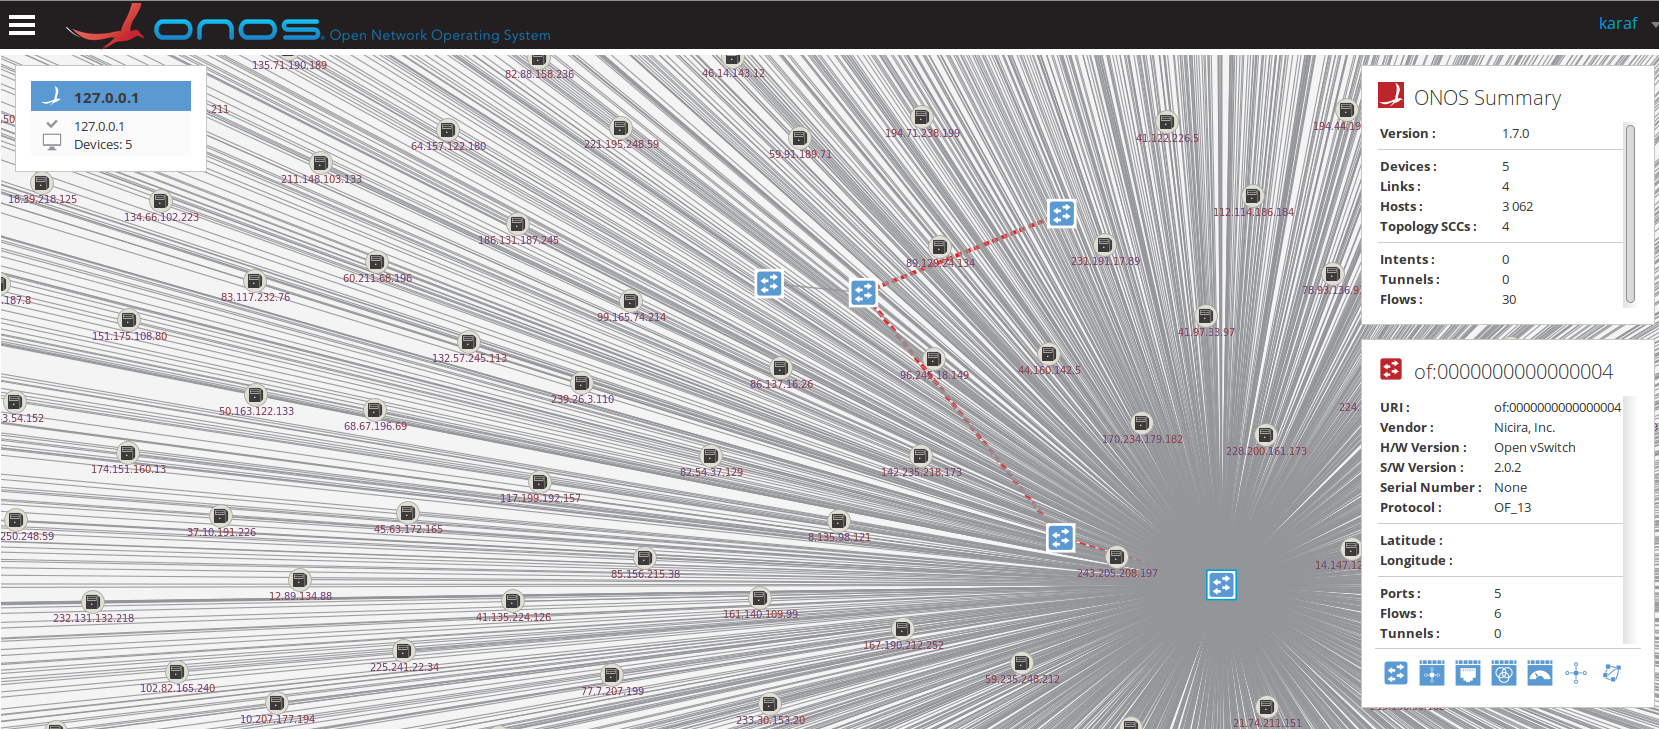
\includegraphics[width=1\textwidth]{surcharge.png}
  	\caption{Réseau attaqué : beaucoup d'hôtes sont détectés par ONOS}
\end{figure}

\begin{figure}[h]
  	\centering
  	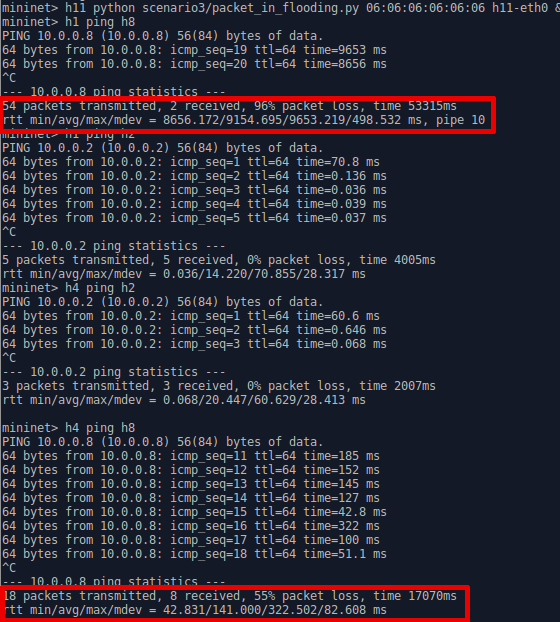
\includegraphics[width=0.7\textwidth]{DOS.png}
  	\caption{Réseau attaqué : ping beaucoup plus faible, perte de paquets}
\end{figure}


Lors de l'attaque, on peut constater que le nombre d'hôtes référencés par ONOS augmente fortement (l'interface graphique fournit alors comme dans l'image précédente une vue assez brouillon du réseau).\\
Sous wireshark, on observe l'échange de nombreux PACKET\_IN et PACKET\_OUT avec le switch malveillant, ainsi que quelques paquets mettant à jour les tables de flux du switch cible.\\
Lorsqu'on ping une machine qui n'est pas reliée au switch cible, les délais sont classiques (quelques millisecondes pour les premiers, puis cela baisse avec l'ajout de règle spécifique à la table de flux). En revanche lorsqu'on ping une machine reliée au switch cible, on perd de nombreux paquets, et les délais sont extrêmement longs.\\
Cela varie évidemment selon la puissance de l'attaque (le délai entre chaque émission de paquet malveillant) et le temps qu'on laisse l'attaque se dérouler (sinon les tables de flux du switch cible contiennent un chemin pour le ping de h1 vers h8 qui ne permet pas de constater la surcharge des tables de flux).

\begin{figure}[h]
  	\centering
  	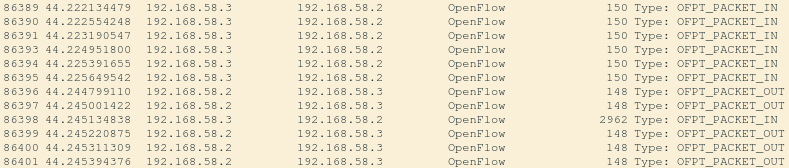
\includegraphics[width=1\textwidth]{packets_in.png}
  	\caption{Nombreux PACKET\_IN et PACKET\_OUT dans ONOS}
\end{figure}
~\\
\underline{Conclusion :}\\
Ce genre d'attaque est présente dans tout réseau (mais spécifique à chaque fois, comme ici "grâce" au mécanisme de PACKET\_IN et à la façon dont se modifie le plan de données en fonction des PACKET\_IN reçus par le contrôleur). Ici, l'attaque réussit en partie car on dispose d'un contrôleur dans sa configuration initiale (qui fait suivre tous les paquets et ajoute des règles pour chaque nouvelle localisation d'hôte détectée).\\
Cela signifie donc qu'en modifiant le comportement par défaut du contrôleur, il est envisageable de réduire fortement les conséquences de la réception de nombreux PACKET\_IN avec des provenances aléatoires. De plus il est assez probable qu'utilisé dans un environnement de production, le contrôleur soit programmé pour aggréger des flux semblables dans des règles communes, factorisant ainsi le traitement de nombreux paquets et empêchant la surcharge des tables de flux (donc l'attaque).
